\documentclass[preview]{standalone}

\usepackage{amsmath}
\usepackage{amssymb}
\usepackage{parskip}
\usepackage{stellar}
\usepackage{fullpage}
\usepackage{hyperref}
\usepackage{blkarray}
\usepackage{tikz}

\hypersetup{
    colorlinks=true,
    linkcolor=black,
    urlcolor=blue,
    pdftitle={Graphs},
    pdfpagemode=FullScreen,
}

\begin{document}

\title{Graphs}
\id{graphs}
\genpage

\section{Definition}

\begin{snippet}{graph-definition}
\sdefinition{Graph}{
    A \textit{graph} is a tuple \((V,E)\) consisting of a set of \textit{vertices} \(V\)
    and a set of \textit{edges} \(E\) where every element in \(E\) is a distinct pair of vertices
    in \(V\).
}
\end{snippet}

\section{Degree}

\begin{snippet}{graph-vertex-degree}
\sdefinition{Graph}{
    Let \(G=(V,E)\) be a graph. The \textit{degree} of a vertex \(v \in V\), denoted \(deg(v)\) is defined
    as the numbers of edges in \(E\) that are incident on \(v\).
}
\end{snippet}

\begin{snippet}{graph-sum-of-degrees}
\sproposition{Sum of degrees of graph}{
    Let \(G=(V,E)\) be a graph.
    The sum of the degrees of all vertices is equals to twice the number of edges.
    \[
        \sum_{v\in V}deg(v)=2|E|
    \]
}
\end{snippet}

\section{Paths}

\begin{snippet}{path-definition}
\sdefinition{Path}{
    Let \(G=(V, E)\) be a graph.
    A \textit{path} on \(G\) is a sequence of vertices in \(V\) connected by edges in \(E\).
}
\end{snippet}

\begin{snippet}{ciclic-path-definition}
\sdefinition{Cycle}{
    Let \(P\) be a path on a graph \(G=(V, E)\).
    The path is said to be \textit{cycle} if it starts and end at the same vertex.
}
\end{snippet}

\begin{snippet}{simple-path-definition}
\sdefinition{Simple path}{
    Let \(P\) be a path on a graph \(G=(V, E)\).
    The path is said to be \textit{simple} if every vertex in it is distinct.
}
\end{snippet}

\begin{snippet}{connected-path-definition}
\sdefinition{Connected path}{
    Let \(G=(V, E)\) be a graph.
    The graph is said to be \textit{connected} if there exist
    at least a path between any pair of vertices.
}
\end{snippet}

\section{Adjacency Matrices}

\begin{snippet}{adjacency-matrix-definition}
\sdefinition{Adjacency Matrix}{
A finite graph can be represented by a square matrix
\(n \times n\) where \(n\) is the number of vertices.

\begin{center}
    \begin{minipage}[r]{6cm}
        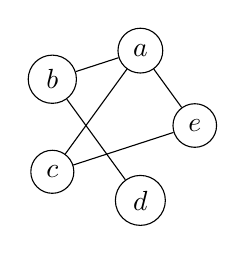
\begin{tikzpicture}[main/.style = {draw, circle}]
            \foreach \x [count = \xi] in {a,b,c,d,e} {
                \node[main] (\xi) at
                    ({1 * cos(360 / 5 * \xi)}, {1 * sin(360 / 5 * \xi)})
                    {\(\x\)};
            }
        
            \draw (1) -- (2);
            \draw (1) -- (3);
            \draw (1) -- (5);
            \draw (2) -- (4);
            \draw (5) -- (3);
        \end{tikzpicture} 
    \end{minipage}
    \begin{minipage}[l]{6cm}
        A=
        \begin{blockarray}{cccccc}
            & a & b & c & d & e \\
            \begin{block}{c(ccccc)}
            a & 0 & 1 & 1 & 0 & 1 \\
            b & 1 & 0 & 0 & 1 & 0 \\
            c & 1 & 0 & 0 & 0 & 1 \\
            d & 0 & 1 & 0 & 0 & 0 \\
            e & 1 & 0 & 1 & 0 & 0 \\
            \end{block}
        \end{blockarray}
    \end{minipage}
\end{center}

Every row and column represents a vertex. \(1\) means
that the two vertices are adjacent, \(0\) otherwise. The diagonal of this matrix
will always e \(0s\) since no vertice is adjacent to itself
and \(A=A^t\)
}
\end{snippet}

\end{document}
